% Section and frames
\section{CHALLENGE OVERVIEW}
\label{challenge_overview_section}

% Section title slide
\sectiontitleframe{CHALLENGE OVERVIEW}

% Slide 1: Introduction to the Challenge
\begin{frame}{Introduction to the Challenge}
    \frametitle{Understanding the House Prices Challenge}
    \begin{itemize}
        \item "House Prices: Advanced Regression Techniques" challenge.
        \item Objective: Predicting house prices using various features.
        \item Real-world relevance: Importance in real estate and economics.      
    \end{itemize}
    \vspace{1.5cm}
    \begin{figure}
        
\includegraphics[width=0.7\textwidth]{figures/housesbanner.png} % Replace 'example-image' with your image file
    \end{figure}
    \vspace{1cm}
    \center
    \tiny
    \textit{Source: "House Price Prediction" \cite{kaggle_house_price_prediction}}
\end{frame}

% Slide 2: Problem Description
\begin{frame}{Problem Description}
    \frametitle{Diving Deeper into the Problem}
    \begin{itemize}
        \item Dataset of residential homes in Ames and Iowa.
        \item 79 explanatory variables for 2919 samples.
        \item Key feature examples: 'LotArea', 'YearBuilt', 'SaleType', etc.
        \item For each Id in the test set, predict the value of the 'SalePrice' variable.
    \end{itemize}
\end{frame}

% Slide 3: Evaluation Methodology
\begin{frame}{Evaluation Methodology}
    \frametitle{Evaluation Criteria}
    \begin{itemize}
        \item Take logarithm of the predicted (\(\hat{y}_i\)) and observed (\(y_i\)) values.
        \item Evaluation metric: Root-Mean-Squared-Error (RMSE) between the logarithms of the predicted and observed sales prices:
    \end{itemize}
    % RMSE formula outside of itemize
    \vspace{0.5cm}
    \begin{equation}
        RMSE = \sqrt{\frac{1}{n}\sum_{i=1}^{n} (\log(\hat{y}_i) - \log(y_i))^2}
        \label{eq:rmse}
    \end{equation}
\end{frame}

% Slide 4: Leaderboard Overview
\begin{frame}{Leaderboard Overview}
    \frametitle{Current Challenge Leaderboard}
    \begin{itemize}
        \item Leaderboard comparison value: RMSE score.
        \item Rank 1 and 2 score < 0.00000.
        \item From rank 3 and 10 score 0.00044 .
    \end{itemize}
    \vspace{0.5cm}
    \begin{figure}
        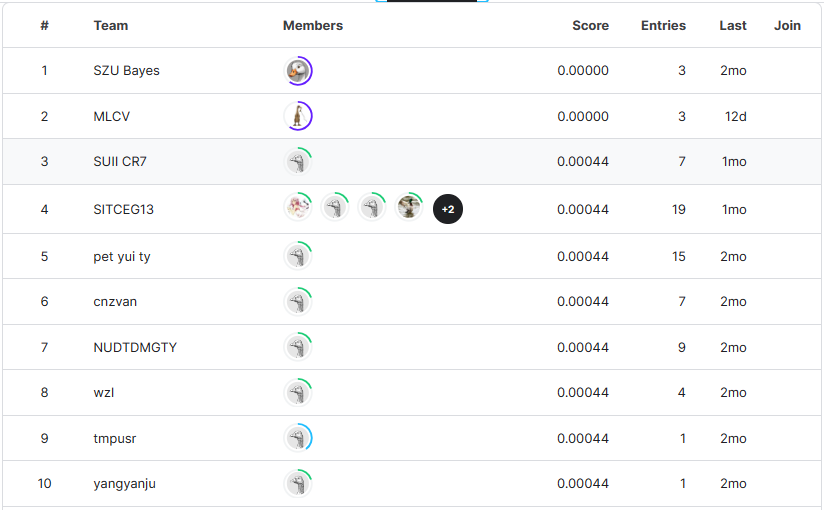
\includegraphics[width=0.5\textwidth]{figures/leaderboard_snapshot.png} 
        \caption{Leaderboard Snapshot.}
        \label{fig:leaderboard_snapshot}
    \end{figure}
\end{frame}

% % Example frame 1
% \begin{frame}{frame} % set section name
%     \frametitle{frame}
%     \begin{itemize}
%         %description:
%         \item 1-2 slides
%         \item Describe the topic (problem) of the challenge; visualise it; describe the reason for considering that problem…
%         %Evaluation
%         \item 1-2 slides
%         \item Describe the evaluation methodology (equations, description, form for official submission); present current leaderboard (up to first 30 participants)…
%     \end{itemize}
% \end{frame}